\section{Basic}

\inputcode{Default Code}{Basic/template.cpp}
\inputcode{.vimrc}{Basic/vimrc}
%\inputcode{Windows Setup}{Basic/windows.tex}
%\inputcode{Debug}{Basic/debug.tex}
\inputcode{Fast IO}{Basic/fastio.cpp}
\inputcode{Random}{Basic/random.cpp}
%\inputcode{Checker}{Basic/checker.sh}
\inputcode{PBDS Tree}{Basic/pbds.cpp}
\inputcode{Pragma}{Basic/pragma.cpp}
\inputcode{SVG Writer}{Basic/SVG.cpp}

\section{Data Structure}

\inputcode{Heavy-Light Decomposition}{DataStructure/HLD.cpp}
%\inputcode{Li-Chao Tree}{DataStructure/LiChao.cpp}
\inputcode{Link Cut Tree}{DataStructure/LinkCutTree.cpp}
\inputcode{Treap}{DataStructure/Treap.cpp}
\inputcode{KD Tree}{DataStructure/KDTree.cpp}
\inputcode{Leftist Tree}{DataStructure/LeftistTree.cpp}
\inputcode{Convex 1D/1D}{DataStructure/Convex1D1D.cpp}
\inputcode{Dynamic Convex Hull}{DataStructure/DynamicConvexHull.cpp}

\section{Flow \& Matching}

\inputcode{Dinic}{Flow_Matching/Dinic.cpp}
\inputcode{Bounded Flow}{Flow_Matching/BoundedFlow.cpp}
\inputcode{MCMF}{Flow_Matching/MCMF.cpp}
\inputcode{Min Cost Circulation}{Flow_Matching/MinCostCirculation.cpp}
\inputcode{Gomory Hu}{Flow_Matching/GomoryHu.cpp}
%\inputcode{ISAP Algorithm}{Flow_Matching/isap.cpp}
\inputcode{Stoer Wagner Algorithm}{Flow_Matching/StoerWagner.cpp}
\inputcode{Bipartite Matching}{Flow_Matching/BipartiteMatching.cpp}
\inputcode{Kuhn Munkres Algorithm}{Flow_Matching/KuhnMunkres.cpp}
\inputcode{Max Simple Graph Matching}{Flow_Matching/MaxSimpleGraphMatching.cpp}
%\inputnote{Stable Marriage}{Flow_Matching/StableMarriage.tex}
\inputnote{Flow Model}{Flow_Matching/Model.tex}
%\inputcode{Weighted General Matching}{Flow_Matching/WeightedGeneralMatching.cpp}

\section{Geometry}

\inputcode{Geometry Template}{Geometry/GeometryTemplate.cpp}
%\inputcode{Convex Hull}{Geometry/ConvexHull.cpp}
\inputcode{Polar Angle Comparator}{Geometry/PolarAngleComp.cpp}
\inputcode{Minkowski Sum}{Geometry/MinkowskiSum.cpp}
\inputcode{Intersection of Circle and Convex Polygon}{Geometry/CircleConvexIntersection.cpp}
\inputcode{Intersection of Circles}{Geometry/CircleCircleIntersection.cpp}
\inputcode{Tangent Line of Circles}{Geometry/CircleCircleTangent.cpp}
\inputcode{Intersection of Line and Convex Polygon}{Geometry/ConvexLineIntersection.cpp}
\inputcode{Intersection of Line and Circle}{Geometry/CircleLineIntersection.cpp}
\inputcode{Point in Circle}{Geometry/PointInCircle.cpp}
\inputcode{Point in Convex}{Geometry/PointInConvex.cpp}
\inputcode{Half Plane Intersection}{Geometry/HalfPlaneIntersection.cpp}
\inputcode{Minimum Enclosing Circle}{Geometry/MinimumEnclosingCircle.cpp}
\inputcode{3D Point}{Geometry/3DPoint.cpp}
\inputcode{ConvexHull3D}{Geometry/ConvexHull3D.cpp}
\inputcode{Delaunay Triangulation}{Geometry/DelaunayTriangulation.cpp}
\inputcode{Voronoi Diagram}{Geometry/VoronoiDiagram.cpp}
\inputcode{Polygon Union}{Geometry/PolyUnion.cpp}
\inputcode{Tangent Point to Convex Hull}{Geometry/TangentPointToHull.cpp}
\inputcode{Heart}{Geometry/Heart.cpp}
\inputcode{Rotating Sweep Line}{Geometry/RotatingSweepLine.cpp}
\inputcode{Vector In Poly}{Geometry/VectorInPoly.cpp}
\inputcode{Convex Hull DP}{Geometry/ConvexHullDP.cpp}
\inputcode{Calculate Points in Triangle}{Geometry/CalcPointsInTriangle.cpp}
%\inputcode{Trapezoidalization}{Geometry/Trapezoidalization.cpp}

\section{Graph}

\inputcode{BCC}{Graph/BCC.cpp}
\inputcode{SCC}{Graph/SCC.cpp}
\inputcode{2-SAT}{Graph/2SAT.cpp}
\inputcode{Dominator Tree}{Graph/DominatorTree.cpp}
\inputcode{Virtual Tree}{Graph/VirtualTree.cpp}
%\inputcode{Directed Minimum Spanning Tree}{Graph/DirectedMST.cpp}
\inputcode{Fast DMST}{Graph/FastDMST.cpp}
\inputcode{Vizing}{Graph/Vizing.cpp}
\inputcode{Maximum Clique}{Graph/MaximumClique.cpp}
\inputcode{Number of Maximal Clique}{Graph/NumberOfMaximalClique.cpp}
\inputcode{Minimum Mean Cycle}{Graph/MinimumMeanCycle.cpp}
\inputcode{Minimum Steiner Tree}{Graph/MinimumSteinerTree.cpp}
\inputcode{Count Cycles}{Graph/CountCycles.cpp}

\section{Math}

\inputcode{Extended Euclidean Algorithm}{Math/ExtGCD.cpp}
\inputcode{Floor \& Ceil}{Math/floor_ceil.cpp}
\inputcode{Legendre}{Math/Legendre.cpp}
\inputcode{Simplex}{Math/Simplex.cpp}
\inputnote{Simplex Construction}{Math/SimplexConstruction.tex}
%\inputcode{Floor Sum}{Math/FloorSum.cpp}
\inputcode{DiscreteLog}{Math/DiscreteLog.cpp}
\inputcode{Miller Rabin \& Pollard Rho}{Math/MillerRabin_PollardRho.cpp}
\inputcode{XOR Basis}{Math/Basis.cpp}
\inputcode{Linear Equation}{Math/LinearEquation.cpp}
\inputcode{Chinese Remainder Theorem}{Math/ChineseRemainderTheorem.cpp}
\inputcode{Sqrt Decomposition}{Math/SqrtDecomposition.cpp}
\inputnote{Floor Sum}{Math/FloorSum.tex}

\section{Polynomial}

\inputcode{FWHT}{Polynomial/FWHT.cpp}
\inputcode{FFT}{Polynomial/FFT.cpp}
\inputcode{NTT}{Polynomial/NTT.cpp}
\inputcode{Polynomial Operation}{Polynomial/PolynomialOperation.cpp}
\inputnote{Generating Function}{Polynomial/GeneratingFunction.tex}
\inputcode{Bostan Mori}{Polynomial/BostanMori.cpp}

\section{String}

\inputcode{KMP Algorithm}{String/KMP.cpp}
\inputcode{Manacher Algorithm}{String/Manacher.cpp}
\inputcode{Lyndon Factorization}{String/Duval.cpp}
\inputcode{Suffix Array}{String/SA.cpp}
\inputcode{Suffix Automaton}{String/SAM.cpp}
\inputcode{Z-value Algorithm}{String/Zvalue.cpp}
\inputcode{Main Lorentz}{String/MainLorentz.cpp}
\inputcode{AC Automaton}{String/Aho_Corasick.cpp}
\inputcode{Palindrome Automaton}{String/PAM.cpp}

\section{Misc}

%\inputcode{Fraction}{Misc/Fraction.cpp}
\inputcode{Cyclic Ternary Search}{Misc/cyc_tsearch.cpp}
\inputnote{Matroid}{Misc/Matroid.tex}
\inputcode{Simulate Annealing}{Misc/SimulateAnnealing.cpp}
\inputcode{Binary Search On Fraction}{Misc/BinarySearchOnFraction.cpp}
\inputcode{Min Plus Convolution}{Misc/MinPlusConvolution.cpp}
\inputcode{SMAWK}{Misc/SMAWK.cpp}
\inputcode{Golden Ratio Search}{Misc/GoldenRatioSearch.cpp}

\section{Notes}

\inputnote{Geometry}{Notes/Geometry.tex}
\inputnote{Trigonometry}{Notes/Trigonometry.tex}
\inputnote{Calculus}{Notes/Calculus.tex}
\inputnote{Sum \& Series}{Notes/SumSeries.tex}
\inputnote{Misc}{Notes/Misc.tex}
\inputnote{Number}{Notes/Number.tex}

\begin{center}
    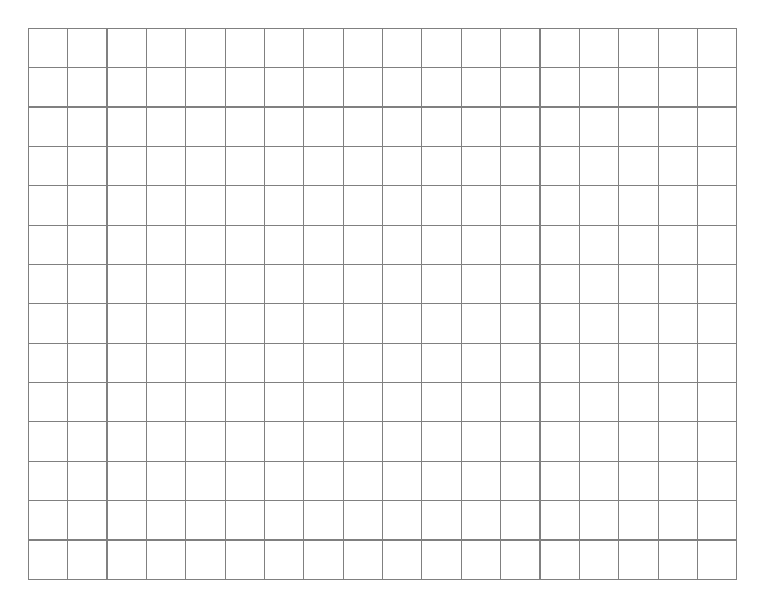
\begin{tikzpicture}
        \draw[step=0.5, gray, thin] (0,0) grid (9.0, 7);
    \end{tikzpicture}
\end{center}

%\onecolumn

%\makegrid
